%
%
%
\subsection{Baseline calibration results {\color{blue} Laurence $\rightarrow$ Juan}}
%\label{se:valid_baseline_cal}

The baseline calibration accuracy and stability are primarily assessed
using two quantities. We define the calibration bias $b$ for array $i$ as
the ratio between the measured flux density $\hat{S_{i}}$ using the
Gaussian fixed-width beam photometry as discussed in
Sect.~\ref{se:cal_HA} and the flux density expectations $\hat{S}$ as
given in Sect.~\ref{se:ref_flux_secondaries}. From a series of
secondary calibrator scans, we evaluate
\begin{itemize}
\item[i)] the average calibration bias per array $b_{\rm A_i}$,
  which by construction, should be equal to unity within the precision
  with which the expected flux densities are known. Moreover, 
  the calibration bias stability against the observed opacity provides
  us with a robustness test of the opacity correction, and the stability
  againts the measured beam size, a test of the photometric
  susceptibility to optical variations. %(driven by the main dish
  %distortions)
\item[ii)] the standard deviation from the mean $\sigma_{\rm A_i}$,
  which consists in an estimate of the statistical calibration
  uncertainties that encloses errors of optical, atmospheric, noise
  and data processing origins. Added in quadrature with the model
  uncertainties reported in Moreno et al., it represents a
  conservative estimate of the total absolute calibration errors.
\end{itemize}


The baseline calibration, discussed in Sect.~\ref{se:baseline_calibration}, is primarily
validated by estimated the flux density of MWC349. In
Fig.~\ref{fig:mwc349_flux_obstau}, we present MWC349
measured-to-expected flux density ratios for the three considered
campaigns and check the ratio stability against the observed opacity,
modeled as the estimated zenith opacity (see Sect.~\ref{se:opacities}) multiplied
by the airmass at the telescope average elevation during the scan. 

\addparag{discussion on the lack of flux at 2mm: 1) calibration error
  of PdB, 2) MWC349 = strong-emission line star: more flux seen at PdB
  ? }

In a broad range of atmospheric conditions, which covers observed opacities from 0.2 to
0.7 at $1~\rm{mm}$, no sizable systematic effects are seen. However, at low observed
opacity ($<0.2$ at $1~\rm{mm}$), flux densities tend to exceed
the average flux densities. This excess reaches about $15\%$ at the
lowest observed opacities that have been probed.

\addparag{discussion on the flux excess at low opacity}

%We conclude that the photometry relying on the baseline
%calibration, is accurate and robust against atmospheric
%conditions.
The detailed results of the calibration validation are
presented in Table~\ref{tab:baseline_calib_result_mwc349}.


\addparag{discussion on the lack of flux at 2mm: 1) calibration error
  of PdB, 2) MWC349 = strong-emission line star: more flux seen at PdB
  ? }


\begin{figure}[ht!]
  \begin{center}
    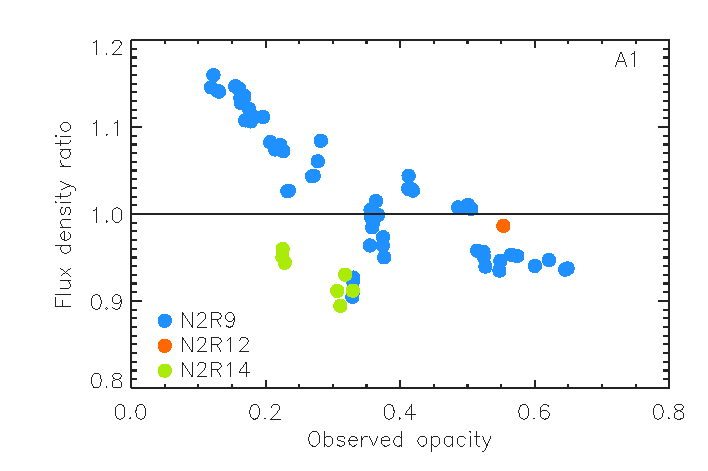
\includegraphics[clip=true,width=0.47\textwidth]{Figures/Calibration/plot_flux_density_ratio_MWC349_obstau_secondary_a1.pdf}
    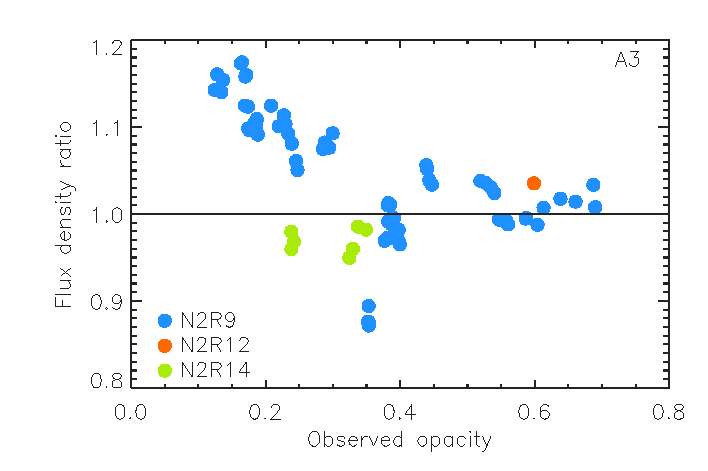
\includegraphics[clip=true,width=0.47\textwidth]{Figures/Calibration/plot_flux_density_ratio_MWC349_obstau_secondary_a3.pdf}
    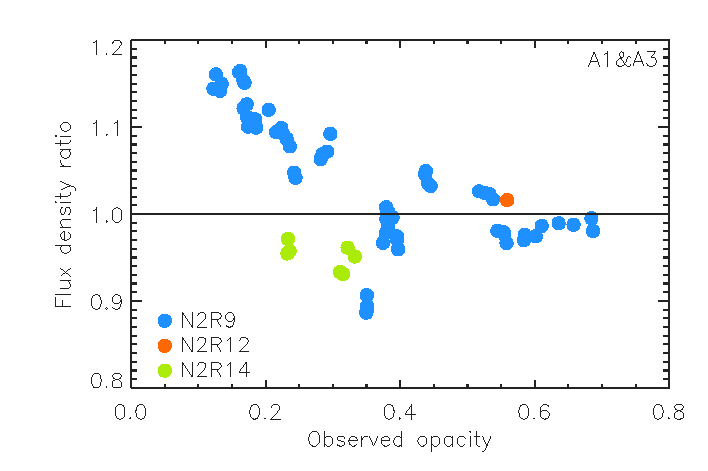
\includegraphics[clip=true,width=0.47\textwidth]{Figures/Calibration/plot_flux_density_ratio_MWC349_obstau_secondary_1mm.pdf}
    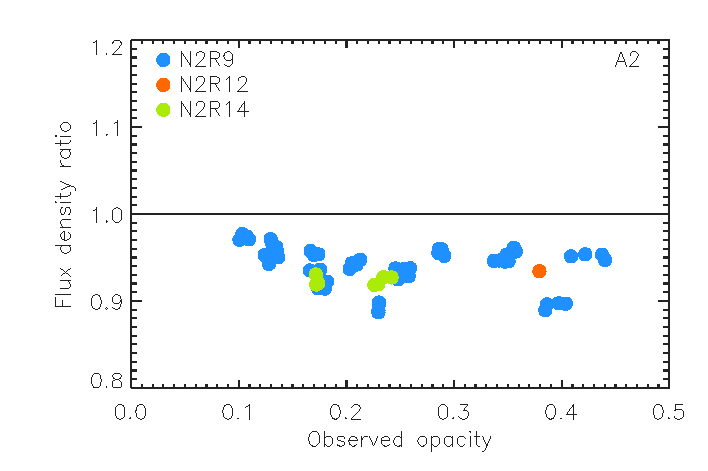
\includegraphics[clip=true,width=0.47\textwidth]{Figures/Calibration/plot_flux_density_ratio_MWC349_obstau_secondary_a2.pdf}
    \caption[MWC349 flux density stability against observed
      opacity]{Measured-to-modeled flux density ratio for the
      secondary calibrator MWC349 as a fonction
      of the measured observed opacity for array 1 (upper left), array 3
      (upper right), 1mm array combination (lower left) and array 2 (lower
      right). The datapoints denote the flux ratio of the scans
      retained after performing the
      baseline selection, for the three campaigns, N2R9
      in blue, N2R12 in orange and N2R14 in chartreuse (yellow
      green). The flux ratios are consistent with unity for the
      $1~\rm{mm}$ observations within $1\sigma$ errors, whereas a
      small but statistically significant discrepancy is observed at
      $2~\rm{mm}$ with respect to the flux expectations from the Plateau
      de Bure (PdB) SED extrapolated in NIKA2 bands. This lack of flux
      w.r.t. PdB, which is stable through the three campaigns, suggesting it
      does not depends on the observing conditions, is further
      discussed in the text.}
    \label{fig:mwc349_flux_obstau}
  \end{center}
\end{figure}



\begin{table}[th]
\begin{center}
\begin{tabular}{|c|c|cccc|}
\hline
Runs & Arrays & $\#$Total scans   & $\#$Selected scans & Flux density bias  & Relative error \\ 
\hline\hline
 N2R9   & A1        & 64                 &  64         & 1.03               &  7.3    \\ 
        & A3        &                    &             & 1.04               &  7.0     \\ 
        & A1$\&$A3  &                    &             & 1.04               &  7.0    \\ 
        & A2        &                    &             & 0.94               &  2.4    \\ 
 \hline
 N2R12  & A1        & 13                 &  1          & 0.99               &  n.a.   \\ 
        & A3        &                    &             & 1.04               &         \\ 
        & A1$\&$A3  &                    &             & 1.02               &         \\ 
        & A2        &                    &             & 0.93               &         \\
 \hline
 N2R14  & A1        & 21                 &  7          & 0.93               &  2.6  \\ 
        & A3        &                    &             & 0.97               &  1.4   \\ 
        & A1$\&$A3  &                    &             & 0.95               &  1.5    \\ 
        & A2        &                    &             & 0.92               &  0.5   \\
 \hline
combined & A1        &  98                & 72         &  1.02              &  7.6  \\ 
         & A3        &                    &            &  1.04              &  7.0  \\ 
         & A1$\&$A3  &                    &            &  1.03              &  7.2   \\ 
         & A2        &                    &            &  0.94              &  2.3  \\
\hline\hline
\end{tabular}
\caption[Baseline calibration results using MWC349]{Baseline
  calibration results using MWC349 photometry. For the observation runs or combination of runs indicated in the first column, we report the total number of observation scans in the third column, the number of scan after the baseline selection in the fourth column, the flux density biases in the fifth, which correspond to the average measured-to-expected flux density ratios, and the relative errors given in percent in the last column, which are the $1\sigma$ errors with respect to the mean flux densities.}
\label{tab:baseline_calib_result_mwc349}
\end{center}
\end{table}


In Fig.~\ref{fig:secondcalib_flux_1_2_mm}, we further check the flux density stability against
the estimated beam size and the atmospheric conditions using other secondary calibrators.

\addparag{CRL2688 and NGC7027}

%We conclude that the photometry relying on the baseline
%calibration, is accurate and robust against atmospheric
%conditions.


\begin{figure}[ht!]
  \begin{center}
    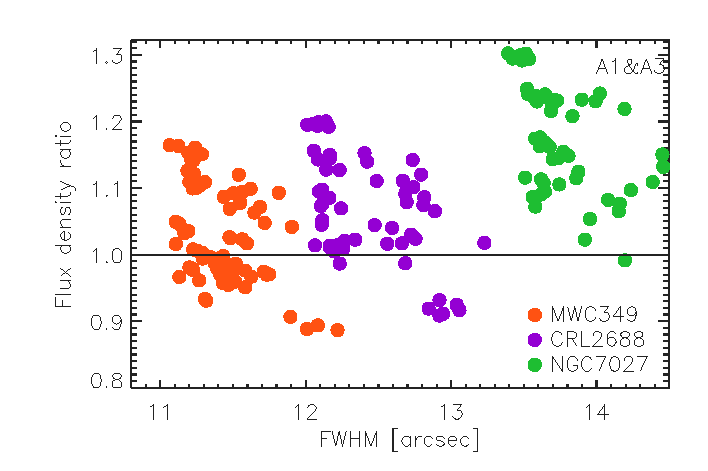
\includegraphics[clip=true,width=0.47\textwidth]{Figures/Calibration/plot_flux_density_ratio_3sources_FWHM_secondary_1mm.pdf}
    \includegraphics[clip=true,width=0.47\textwidth]{Figures/Calibration/plot_flux_density_ratio_3sources_FWHM_secondary_a2.pdf}
    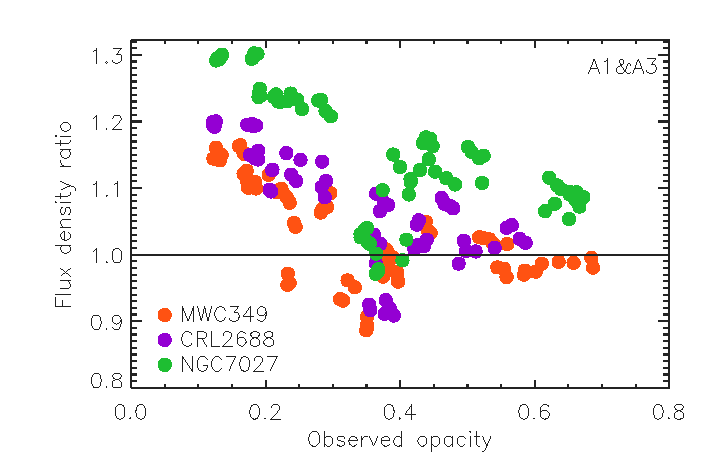
\includegraphics[clip=true,width=0.47\textwidth]{Figures/Calibration/plot_flux_density_ratio_3sources_obstau_secondary_1mm.pdf}
    \includegraphics[clip=true,width=0.47\textwidth]{Figures/Calibration/plot_flux_density_ratio_3sources_obstau_secondary_a2.pdf}
    \caption[Flux density stability against observing conditions using
      secondary calibrators]{Measured-to-modeled flux density ratio
      for the three considered secondary calibrators as a function of
      the measured FWHM (upper plots) and the observed opacity
      (lower plots) at $1~\rm{mm}$ (left) and $2~\rm{mm}$ (right).
      Datapoints denote the flux ratio of MWC349 in orange, CRL2688 in
      violet and NGC7027 in green.
      Whereas MWC349 is point-like in NIKA2 bands, CRL2688 is slightly
      extended and the planetary nebulea NGC7027 partly resolved. The
      latter is thus less suited to check point-source
      photometry. CRL2688 has flux ratios consistent with unity in both
      NIKA2 bands: NIKA2 measurements for this secondary calibrator
      are in excellent agreement with SCUBA2 flux estimates. In
      addition, flux ratios are constant within statistical
      uncertainties against both the beam size and the observed
      opacity.}
    \label{fig:secondcalib_flux_1_2_mm}
  \end{center}
\end{figure}
